\chapter{Elements of Probability}


\begin{flushright}
	\textit{``You have to look at it from a Bayesian perspective."} 
\end{flushright}

\textbf{Interpretations of Probability} : A probability can be understood as either an inference based on many observations of similar events in the past, or as a quantitative estimate of the experimenter's belief in a hypothesis.

\textit{Frequentist} : Repeating the same experiment many times and observing the set of all outcomes enables one to assign a probability to a future outcome of that experiment as a property attached to the outcome itself. This probability is independent of the observer and is an inherent feature of the outcome and the underlying experiment.

\textit{Subjective / Bayesian} : This is a number indicating a person's belief in the outcome and is inherently subjective. Common in philosophy and economic theory.

\textbf{Sample Space} : set of all possible outcomes of an experiment (denoted by $ S $). An \textit{event} is a subset of the sample space containing one or more elements. It is commonly used to denote the outcome of an experiment.

The union of two events ($ E \cup F $) as well as their intersection ($ E \cap F $) are defined using the usual set theory norms. An intersection of two events with no common elements is the null event $ \varnothing $ (same notation as null set).

If $ E \cap F = \varnothing $, the events E and F are called \textit{mutually exclusive}.

From set theory, the complement of an event is the set of all elements in the sample space not contained in the event. $ E^{\complement}  = S - E$, making an event mutually exclusive with its complement. It follows that $ S^{\complement} = \varnothing $.

If one event contains all of the elements of another, then they are related by a subset-superset relationship. This is denoted by $ E \subset F $ or by $ F \supset E $. When two events are subsets of each other, they are considered identical or equal events.

\begin{align}
	\text{If} \qquad E \subset F \qquad \text{and} \qquad F \subset E \qquad \text{then, } \qquad E = F
\end{align}

Boolean algebra may be invoked to define the set operations on more than two events, as an extension of the above. The basic associative law, commutative law and distributive law of sets applies here to events trivially.

\textit{De-Morgan's Law} is a useful relation between the complements of unions or intersections of sets. 

\begin{align}
	(E \cup F)^{\complement} &= E^\complement \cap F^\complement \\
	%
	(E \cap F)^{\complement} &= E^\complement \cup F^\complement 
\end{align}

The above relations can be verified using \textit{Venn Diagrams}, which are the easiest way to graphically represent set algebra.

\textbf{Axioms of Probability} : For any experiment repeatedly conducted under identical conditions, the probability of an event will approach a fixed number asymptotically. This is the empirical probability ($ P $) of that event.

\begin{align}
	0 \leq P(E) \leq 1 \\
	%
	P(S) = 1 
\end{align}

For a set of mutually exclusive events $ \{ E_i \} $, 

\begin{align}
	P \left( \bigcup_{i = 1}^{n} E_i \right) &= \sum\limits_{i = 1}^{n} P(E_i) \\
	%
	P \left( \bigcap_{i = 1}^{n} E_i \right) &= 0
\end{align}

Using the fact that an event is mutually exclusive with its complement, 

\begin{align}
	P(E^\complement) = 1 - P(E)
\end{align}

\begin{figure}[H]
	\centering
	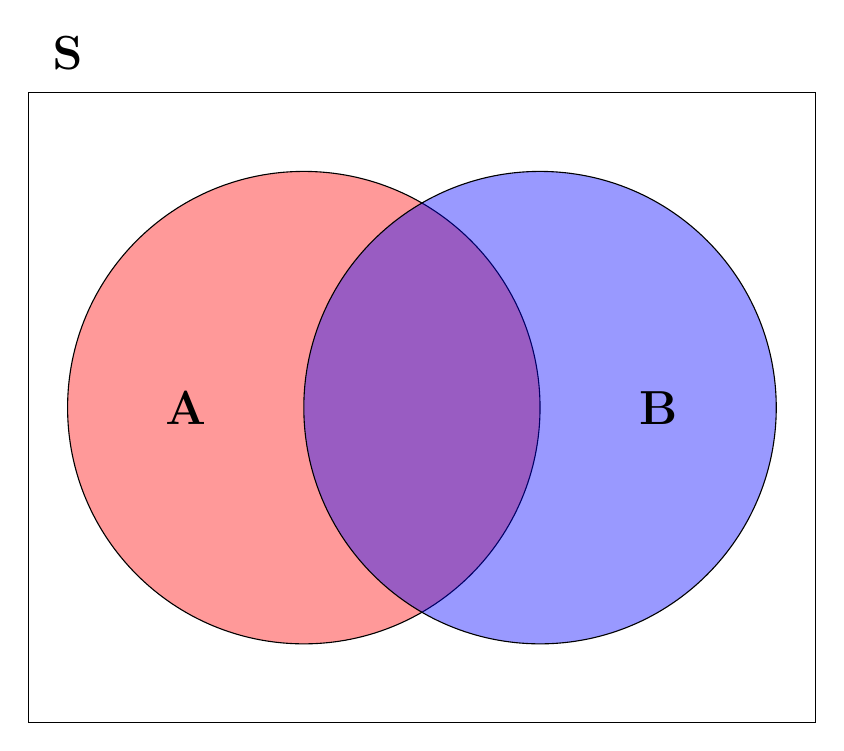
\begin{tikzpicture}
		%% You can adjust the opacity here. For venn diagrams it is convenient to have a low opacity so that you can see intersections
		\begin{scope} [fill opacity = .4]
			%% The draw command knows a lot of shapes. To make a rectangle you just need to specify two diagonal corners. Make sure you always have a semicolon at the end of your draw commands, otherwise latex flips out.
			\draw (-5,4) rectangle (5,-4);
			%% Similarly, you can make a circle by specifying the center and then the radius. You can also add a fill color, but if you're printing in black and white you'll probably want to remove that line.
			\draw[fill=red, draw = black] (-1.5,0) circle (3);
			\draw[fill=blue, draw = black] (1.5,0) circle (3);
			%% We can use the node command to label points. If you put your cursor on "LARGE" or "textbf" a box will drop down with size and text style options.
			\node at (-4.5,4.5) [text opacity = 1] {\LARGE\textbf{S}};
			\node at (-3,0) [text opacity = 1] {\LARGE\textbf{A}};
			\node at (3,0) [text opacity = 1] {\LARGE\textbf{B}};
		\end{scope}
		%% And now you have a venn diagram. Yay!
		%\draw[help lines](-5,5) grid (5,-6);    This line can draw the grid lines to help guide you. I use these when I'm writing the code and then delete this line when I publish the pdf.
	\end{tikzpicture}
	\caption{The purple area at the intersection of A and B is counted twice when naively adding the areas of A and B.} 
\end{figure} 

The probability of $ E \cup F $ is not the naive sum of the two individual probabilities, as seen in the Venn diagram here.

\begin{align}
	P(E \cup F) = P(E) + P(F) - P(E \cap F)
\end{align}

\textit{Odds} : the odds of an event is defined as a measure how much more likely an event is to occur compared to its complement. 

\begin{align}
	\frac{P(A)}{P(A^\complement)} = \frac{P(A)}{1 - P(A)}
\end{align}

\textbf{Equally likely outcomes} : It is common in real world experiments that every element of the sample space is equally likely. (Dice roll, coin flip, Lottery etc.). This special case simplifies the probability of an event to : 

\begin{align}
	P(E) = \frac{\text{number of element in E}}{\text{number of total elements}}
\end{align}

\textbf{Basic principles of counting} : For $ k $ repetitions of an experiment each with outcomes $ \{ n_1, n_2, ...., n_k \} $ respeectively, the total number of outcomes of the set of $ k $ repetitions is $ \left( \prod n_i  \right)$ 

\textit{Permutation} : The number of ways of selecting $ k $ out of $ n $ elements with sequence being relevant.

\begin{align}
	\Myperm{k} = \frac{n!}{(n-k)!} = \Mycomb{k} \ k! 
\end{align}

\textit{Combination} : The number of ways of selecting $ k $ out of $ n $ elements without regard to sequence. By convention, $ \Mycomb{0} = 1 $, using the fact that $ 0! = 1 $

\begin{align}
	\Mycomb{k} = \frac{n!}{(n-k)! \ k!} = \binom{n}{k}
\end{align}

\textbf{Conditional probability} : Useful when part of the outcome is known but not the full details. It looks at the probability of one event ($ A $) occurring, given another event ($ B $) has occurred. If the event $ B $ has occurred, then the sample space is now $ B $ instead of the initial $ S $. The desirable set of events now becomes the subset of elements in $ A $ that also happen to be in $ B $. This leads to the definition :

\begin{align}
	P(A|B) = \frac{P(A \cap B)}{P(B)}
\end{align}

Rearranging the above definition provides a convenient way to calculate the probability of the intersection of two events. 

\begin{align}
	P(A \cap B) = P(A|B)\ P(B)
\end{align}

\textbf{Bayes' theorem} : To find the probability of an event occurring, it is often useful to 'condition' it on the occurrence of another event. Using the definition of the complement of an event, 

\begin{align}
	P(A) &= P(A \cap B) + P(A \cap B^\complement) \\
	%
	P(A) &= P(A|B)\ P(B) + P(A|B^\complement)\ P(B^\complement)\\
	%
	P(A) &= P(B) \ P(A|B) + (1 - P(B))\ P(A|B^\complement)
\end{align}

Note that $ P(A) $ above becomes a linear interpolation between the two edges $ P(A|B) $ and $ P(A|B^\complement) $ with the sliding parameter being $ P(B) $. This is a useful perspective for many real-world problems.

An important pillar of Bayesian probability is the notion of updating a prior probability estimate after incorporating new (usually incomplete) information about the outcome.

The generalization of the conditional probability formula to more than two events is called Bayes' theorem. Let the set of mutually exclusive events $ \{ B_i \} $ be such that exactly one of them must occur.

\begin{align}
	\bigcup_{i = 1}^{n} B_i &= S \qquad \text{and} \qquad B_i \cap B_j = \varnothing \quad \forall \quad i \neq j \\
	%
	P(B_k|A) &= \frac{P(A \cap B_k)}{P(A)} = \frac{P(A | B_k) \ P(B_k)}{\sum_{i}P(A | B_i) \ P(B_i)}
\end{align}

The historical use of this formula was to update the probabilities of various hypotheses $ {B_i} $ after an experiment provides additional evidence $ A $.

\textbf{Independent events} : Two events are independent if the occurrence of one event does not affect the occurrence of the other event. 

\begin{align}
	P(A \cap B) &= P(A) \ P(B) \\
	%
	P(A|B) &= \frac{P(A \cap B)}{P(B)} = P(A)
\end{align}

If $ A $ and $ B $ are independent events, then so are $ A $ and $ B^\complement $. The above result extends to more than two events if any possible subset of the events is also independent. 

\newpage

